\chapter{The CHIPS experiment}
\label{chap:chips}

\chapterquote{There, sir! that is the perfection of vessels!}
{Jules Verne, 1828--1905}

\section{The \CHIPS Concept}
The CHerenkov detectors In mine PitS (\CHIPS) research and development project is a
new way of approaching accelerator neutrino experiments.


\begin{figure}
    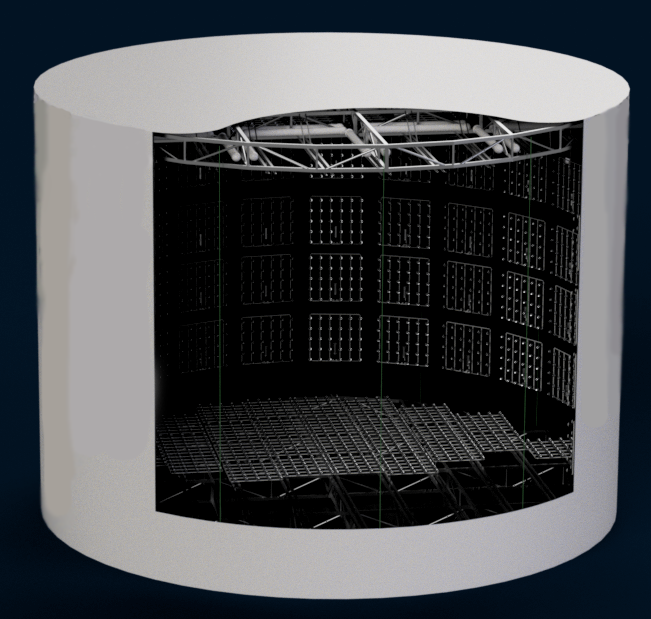
\includegraphics[width=\largefigwidth]{diagrams/chips/chips_render_1}
    \caption[CKM Fitter constraints on \alphaCKM.]%
    {CKM Fitter constraints on \alphaCKM from combined \BToPiPi,
        \BToRhoPi and \BToRhoRho decay analyses.}
    \label{fig:chips_render_1}
\end{figure}

\begin{figure}
    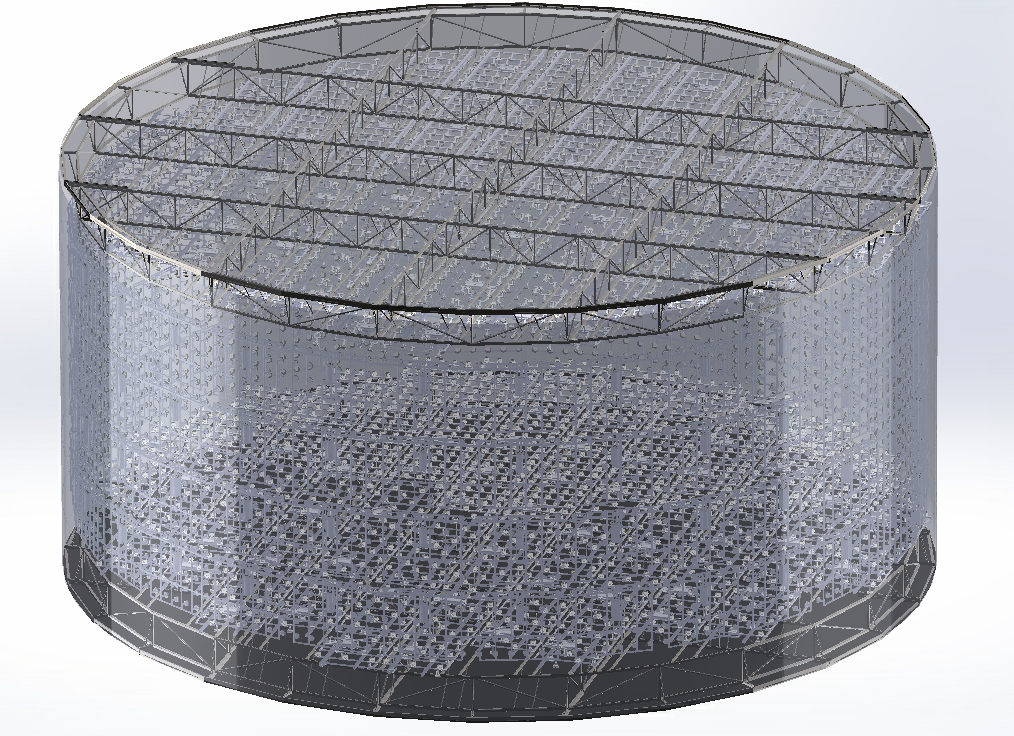
\includegraphics[width=\largefigwidth]{diagrams/chips/chips_render_2}
    \caption[CKM Fitter constraints on \alphaCKM.]%
    {CKM Fitter constraints on \alphaCKM from combined \BToPiPi,
        \BToRhoPi and \BToRhoRho decay analyses.}
    \label{fig:chips_render_2}
\end{figure}


\section{A Detailed look at \CHIPS}
\label{sec:detailedchips}

Since both \bhadron{s} are preferentially produced in the same direction
and are forward-boosted along the beam-pipe, the detector is not required
to have full $4\pi$ solid-angle coverage. \LHCb takes advantage of this
by using a wedge-shaped single-arm detector with angular acceptance
\unit{10-300}{\mrad} in the horizontal (bending) plane~\cite{Amato:1998xt}.

\vspace{1cm}

\begin{center}
    {\hspace{1mm}\Large\vdots\hspace{1cm}}
\end{center}

\vspace{1cm}

The detector is illustrated in \FigureRef{fig:chips_render_1}, showing
the overall scale of the experiment.

\begin{sidewaysfigure}
    \begin{center}
        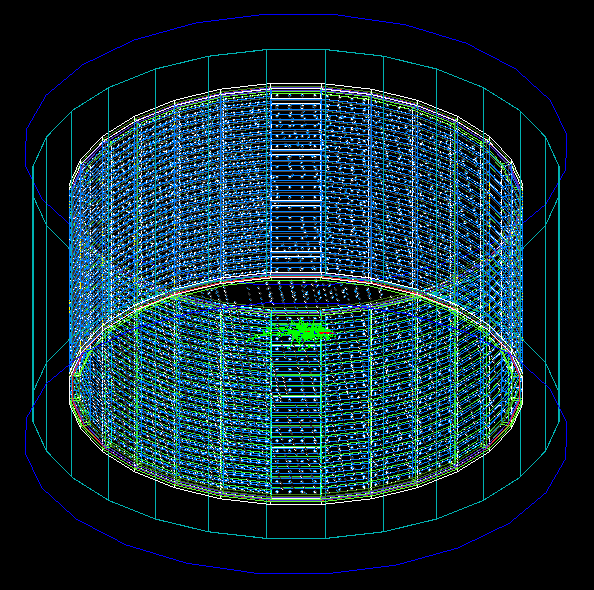
\includegraphics[width=0.8\textheight]{diagrams/chips/chips_event}
        \caption[Cross-section view of \LHCb, cut in the non-bending $y$--$z$ plane]%
        {Cross-section view of \LHCb, cut in the non-bending $y$--$z$ plane.}
        \label{fig:chips_event}
    \end{center}
\end{sidewaysfigure}

The single-sided detector design was chosen in preference to a two-armed
design since the detector dimensions are restricted by the layout of the
IP8 (ex-Delphi) cavern in which \LHCb is located. Using all the available
space for a single-arm spectrometer more than compensates in performance
for the \about{50\percent} drop in luminosity.

\section{The \Cerenkov mechanism}
A Huygens construction in terms of spherical shells of probability for photon
emission as the particle progresses along its track shows an effective
``shock-front'' of \Cerenkov emission. This corresponds to an emission cone of
opening angle \thetaCerenkov around the momentum vector for each point on the
track,
%
\begin{subequations}
    \label{eq:cosThetaCk}
    \begin{equation}
        \cos\,\thetaCerenkov  &= \frac{1}{n \beta} +
        \frac{\hbar k}{2p}%
        \parenths{ 1 - \frac{1}{n^2} } \\
        &\,\sim \frac{1}{n \beta}%
        \label{eq:cosThetaCkApprox}
    \end{equation}
\end{subequations}
%
where $\beta \equiv v/c$, the relativistic velocity fraction.

\section{Trigger system}
\label{sec:triggers}
An overview of the \LHCb trigger characteristics broken down by level
is shown in \Table~\ref{tab:TriggerDetails}.

\begin{table}[bp]
    \begin{tabular}{lllll}
                    & L0              & L1              & HLT             \\
        \midrule                                                          \\
        Input rate  & \unit{40}{\MHz} & \unit{1}{\MHz}  & \unit{40}{\kHz} \\
        Output rate & \unit{1}{\MHz}  & \unit{40}{\kHz} & \unit{2}{\kHz}  \\
        Location    & On detector     & Counting room   & Counting room   \\
    \end{tabular}
    \caption{Characteristics of the trigger levels and offline analysis.}
    \label{tab:TriggerDetails}
\end{table}
